\section{Formation Path Following}
\label{sec:background_formation_path_following}

This section formally defines the formation path following problem.
Throughout the section, we consider a fleet of $N$ vehicles.
Let $\mat{p}_1, \ldots, \mat{p}_N$ denote the positions of the vehicles.

\subsection{The path-following problem}
To formulate the path-following problem, we first need to define the \emph{barycenter} of the fleet.
The barycenter, $\mat{p}_b$, is given by the mean position of the vehicles, \emph{i.e.,}
\begin{equation}
    \mat{p}_b = \frac{1}{N} \sum_{i=1}^N \mat{p}_i.
    \label{eq:background_p_b}
\end{equation}

To solve the path-following problem, we need to control the vehicles such that the barycenter coincides with the desired path.
Let $\mat{p}_p(s)$ be the parametrization of the desired path.
Then, the goal of path-following is to control the vehicles such that
\begin{equation}
    \mat{p}_b \rightarrow \mat{p}_p(s).
\end{equation}

Let $\mat{p}_b^p$ denote the position of the barycenter in the path-tangential coordinate frame (see Section~\ref{sec:background_path_tangential}).
\begin{equation}
    \mat{p}_b^p = \mat{R}_p\T \left(\mat{p}_b - \mat{p}_p(s)\right).
\end{equation}
Note that $\mat{p}_b^p$ can be interpreted as the path-following error.
Indeed, $\mat{p}_b$ is equal to $\mat{p}_p(s)$ if and only if $\mat{p}_b^p$ is zero.

Furthermore, there is a geometric interpretation of the components of $\mat{p}_b^p$.
Let us define $\inlinevector{x_b^p, y_b^p, z_b^p} = \mat{p}_b^p$.
The component $x_b^p$ is commonly referred to as the \emph{along-track error}, since the value of $x_b^p$ indicates whether the barycenter is ``in front of'' or ``behind'' the desired path.
The components $y_b^p$ and $z_b^p$ are referred to as the \emph{cross-track errors}, since they indicate the lateral deviation from the desired path.

\subsubsection{Path-following versus trajectory-tracking}
In the remainder of this section, we discuss the difference between the trajectory-tracking and the path-following problem.

The goal of trajectory tracking is to control the vehicles such that the barycenter follows a given trajectory $\mat{p}_d(t)$.
Note that the desired trajectory is a function of time.
Consequently, in trajectory tracking, the desired position of the barycenter for a given time $t$ is fixed.
In path following, the desired position of the barycenter depends on the path parameter $s$.
The path parameter can be treated as an additional degree of freedom when designing the path-following controller.

\subsection{The formation-keeping problem}
\label{sec:background_formation_keeping}
The \emph{formation} is defined by the relative positions of the vehicles.
Let
\begin{equation}
    \mat{p}_{{\rm rel}, i} = \mat{p} - \mat{p}_b,
    \label{eq:background_p_rel}
\end{equation}
denote the relative position of vehicle $i$.
The goal of formation-keeping is to control the vehicles such that
\begin{align}
    &\mat{p}_{{\rm rel}, i} \rightarrow \mat{p}_{f, i}, &
    & \forall i = 1, \ldots, N,
\end{align}
where $\mat{p}_{f, 1}, \ldots, \mat{p}_{f, N}$ are vectors that represent the desired formation.

From \eqref{eq:background_p_b} and \eqref{eq:background_p_rel}, the sum of the relative positions is
\begin{equation}
    \sum_{i=1}^N \mat{p}_{{\rm rel}, i} = \sum_{i=1}^N \left(\mat{p}_i - \frac{1}{N}\sum_{j=1}^N \mat{p}_j \right) = \mat{0}.
\end{equation}
Consequently, to make the formation-keeping problem feasible, the vectors $\mat{p}_{f, 1}, \ldots, \mat{p}_{f, N}$ must be chosen such that
\begin{equation}
    \sum_{i=1}^N \mat{p}_{f, i} = \mat{0}.
\end{equation}

Formations can be split into two categories: static and dynamic.
In \emph{static} formations, the vectors $\mat{p}_{f, i}$ are constant.
In \emph{dynamic} formations, the vectors $\mat{p}_{f, i}$ are time-varying.
In this thesis, we investigate a specific type of dynamic formations: formations that rotate with the desired path.
In this type of formation, the desired relative positions are given by
\begin{align}
    \mat{p}_{f, i} &= \mat{R}_p(s) \mat{p}_{f, i}^f,&
    i &= 1, \ldots, N,
\end{align}
where $\mat{p}_{f, i}^f$ is a constant vector.

\pgfplotsset{table/search path={figures/background/data}}
\begin{figure}[t]
    \centering
    \begin{subfigure}{0.48\textwidth}
        \centering
        \definecolor{mycolor1}{rgb}{0.00000,0.44700,0.74100}%
\definecolor{mycolor2}{rgb}{0.85000,0.32500,0.09800}%

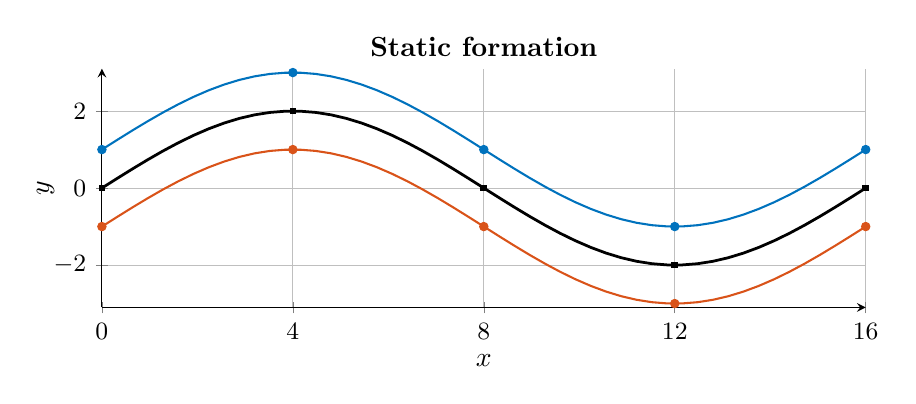
\begin{tikzpicture}
\begin{axis}[
    width=0.8\textwidth,
    height=0.25\textwidth,
    scale only axis,
    axis lines=left,
    xlabel=$x$,
    xlabel style={yshift=0.5mm},
    ylabel=$y$,
    ylabel style={yshift=-2.5mm},
    xmin=0,
    xmax=16,
    xtick={0,4,8,12,16},
    ymin=-3.1,
    ymax=3.1,
    xmajorgrids,
    ymajorgrids,
    title style={font=\bfseries, yshift=-1.75mm},
    title={Static formation},
    tick label style={font=\small},
]

\addplot[
    domain=0:16,
    samples=51,
    color=black,
    line width=1pt,
]
{2*sin((180/8)*x)};

\addplot[
    domain=0:16,
    samples=51,
    color=mycolor1,
    line width=0.75pt,
]
{2*sin((180/8)*x) + 1};

\addplot[
    domain=0:16,
    samples=51,
    color=mycolor2,
    line width=0.75pt,
]
{2*sin((180/8)*x) - 1};

\addplot[only marks, mark size=1pt, mark=square*, draw=black, fill=black]
table {
    0 0
    4 2
    8 0
    12 -2
    16 0
};

\addplot[only marks, mark size=1.5pt, mark=*, draw=mycolor1, fill=mycolor1]
table {
    0 1
    4 3
    8 1
    12 -1
    16 1
};

\addplot[only marks, mark size=1.5pt, mark=*, draw=mycolor2, fill=mycolor2]
table {
    0 -1
    4 1
    8 -1
    12 -3
    16 -1
};
    
\end{axis}
\end{tikzpicture}        
        \vspace*{-1.75em}
        \caption{Example of a static formation.}
        \label{fig:background_formation_static}
    \end{subfigure}
    \begin{subfigure}{0.48\textwidth}
        \centering
        \definecolor{mycolor1}{rgb}{0.00000,0.44700,0.74100}%
\definecolor{mycolor2}{rgb}{0.85000,0.32500,0.09800}%

\begin{tikzpicture}
\begin{axis}[
    width=0.8\textwidth,
    height=0.25\textwidth,
    scale only axis,
    axis lines=left,
    xlabel=$x$,
    xlabel style={yshift=0.5mm},
    ylabel=$y$,
    ylabel style={yshift=-2.5mm},
    xmin=-0.7,
    xmax=16.7,
    xtick={0,4,8,12,16},
    ymin=-3.1,
    ymax=3.1,
    xmajorgrids,
    ymajorgrids,
    title style={font=\bfseries, yshift=-2.75mm},
    title={Dynamic formation},
    tick label style={font=\small},
]

\addplot[
    domain=-1:17,
    samples=51,
    color=black,
    line width=1pt,
]
{2*sin((180/8)*x)};

\addplot[
    color=mycolor1,
    line width=0.75pt,
]
table{formation_dynamic_1.tsv};

\addplot[
    color=mycolor2,
    line width=0.75pt,
]
table{formation_dynamic_2.tsv};

\addplot[only marks, mark size=1pt, mark=square*, draw=black, fill=black]
table {
    0 0
    4 2
    8 0
    12 -2
    16 0
};

\addplot[only marks, mark size=1.5pt, mark=*, draw=mycolor1, fill=mycolor1]
table {
    -0.6170    0.7870
    4.0001    2.9974
    8.6177    0.7864
   12.0001   -0.9986
   15.3830    0.7869
};

\addplot[only marks, mark size=1.5pt, mark=*, draw=mycolor2, fill=mycolor2]
table {
    0.6170   -0.7869
    3.9999    0.9986
    7.3823   -0.7864
   11.9999   -2.9974
   16.6170   -0.7870
};
    
\end{axis}
\end{tikzpicture}        
        \vspace*{-1.75em}
        \caption{Example of a dynamic formation.}
        \label{fig:background_formation_dynamic}
    \end{subfigure}
    \vspace*{-0.5em}
    \caption{Examples of a static and a dynamic formation. The black line represents the desired path, the blue and red lines represent the desired positions of the vehicles. The markers represent the desired positions for $s = 0, 4, \ldots, 16$.}
    \label{fig:background_formation}
\end{figure}

An example of a static and a dynamic formation is shown in \figref{fig:background_formation}.
In both cases, the barycenter should follow a sine-wave path that can be parametrized, \emph{e.g.,} by
\begin{equation}
    \mat{p}_p(s) = \inlinevector{s, 2 \sin\left(\frac{\pi}{8} s\right)}.
\end{equation}
\figref{fig:background_formation_static} shows a static formation consisting of two vehicles, with the desired relative positions given by
\begin{align}
    \mat{p}_{f,1} &= \inlinevector{0, 1}, &
    \mat{p}_{f,2} &= \inlinevector{0, -1}.
\end{align}
\figref{fig:background_formation_static} shows a dynamic formation that rotates with the desired path.
The formation consists of two vehicles with the desired relative positions given by
\begin{align}
    \mat{p}_{f, i} &= \mat{R}_p(s) \mat{p}_{f, i}^f, &
    \mat{p}_{f,1}^f &= \inlinevector{0, 1}, &
    \mat{p}_{f,2}^f &= \inlinevector{0, -1}.
\end{align}
